\documentclass[11pt,a4paper]{report}
\usepackage[textwidth=37em,vmargin=30mm]{geometry}
\usepackage{calc,xunicode,amsmath,amssymb,paralist,enumitem,tabu,booktabs,datetime2,xeCJK,xeCJKfntef,listings}
\usepackage{tocloft,fancyhdr,tcolorbox,xcolor,graphicx,eso-pic,xltxtra,xelatexemoji}

\newcommand{\envyear}[0]{2025}
\newcommand{\envdatestr}[0]{2025-07-26}
\newcommand{\envfinaldir}[0]{webdb/2025/20250726/final}

\usepackage[hidelinks]{hyperref}
\hypersetup{
    colorlinks=false,
    pdfpagemode=FullScreen,
    pdftitle={Web Digest - \envdatestr}
}

\setlength{\cftbeforechapskip}{10pt}
\renewcommand{\cftchapfont}{\rmfamily\bfseries\large\raggedright}
\setlength{\cftbeforesecskip}{2pt}
\renewcommand{\cftsecfont}{\sffamily\small\raggedright}

\setdefaultleftmargin{2em}{2em}{1em}{1em}{1em}{1em}

\usepackage{xeCJK,xeCJKfntef}
\xeCJKsetup{PunctStyle=plain,RubberPunctSkip=false,CJKglue=\strut\hskip 0pt plus 0.1em minus 0.05em,CJKecglue=\strut\hskip 0.22em plus 0.2em}
\XeTeXlinebreaklocale "zh"
\XeTeXlinebreakskip = 0pt


\setmainfont{Brygada 1918}
\setromanfont{Brygada 1918}
\setsansfont{IBM Plex Sans}
\setmonofont{JetBrains Mono NL}
\setCJKmainfont{Noto Serif CJK SC}
\setCJKromanfont{Noto Serif CJK SC}
\setCJKsansfont{Noto Sans CJK SC}
\setCJKmonofont{Noto Sans CJK SC}

\setlength{\parindent}{0pt}
\setlength{\parskip}{8pt}
\linespread{1.15}

\lstset{
	basicstyle=\ttfamily\footnotesize,
	numbersep=5pt,
	backgroundcolor=\color{black!5},
	showspaces=false,
	showstringspaces=false,
	showtabs=false,
	tabsize=2,
	captionpos=b,
	breaklines=true,
	breakatwhitespace=true,
	breakautoindent=true,
	linewidth=\textwidth
}






\newcommand{\coverpic}[2]{
    % argv: itemurl, authorname
    Cover photo by #2~~(\href{#1}{#1})
}
\newcommand{\makeheader}[0]{
    \begin{titlepage}
        % \newgeometry{hmargin=15mm,tmargin=21mm,bmargin=12mm}
        \begin{center}
            
            \rmfamily\scshape
            \fontspec{BaskervilleF}
            \fontspec{Old Standard}
            \fontsize{59pt}{70pt}\selectfont
            WEB\hfill DIGEST
            
            \vfill
            % \vskip 30pt
            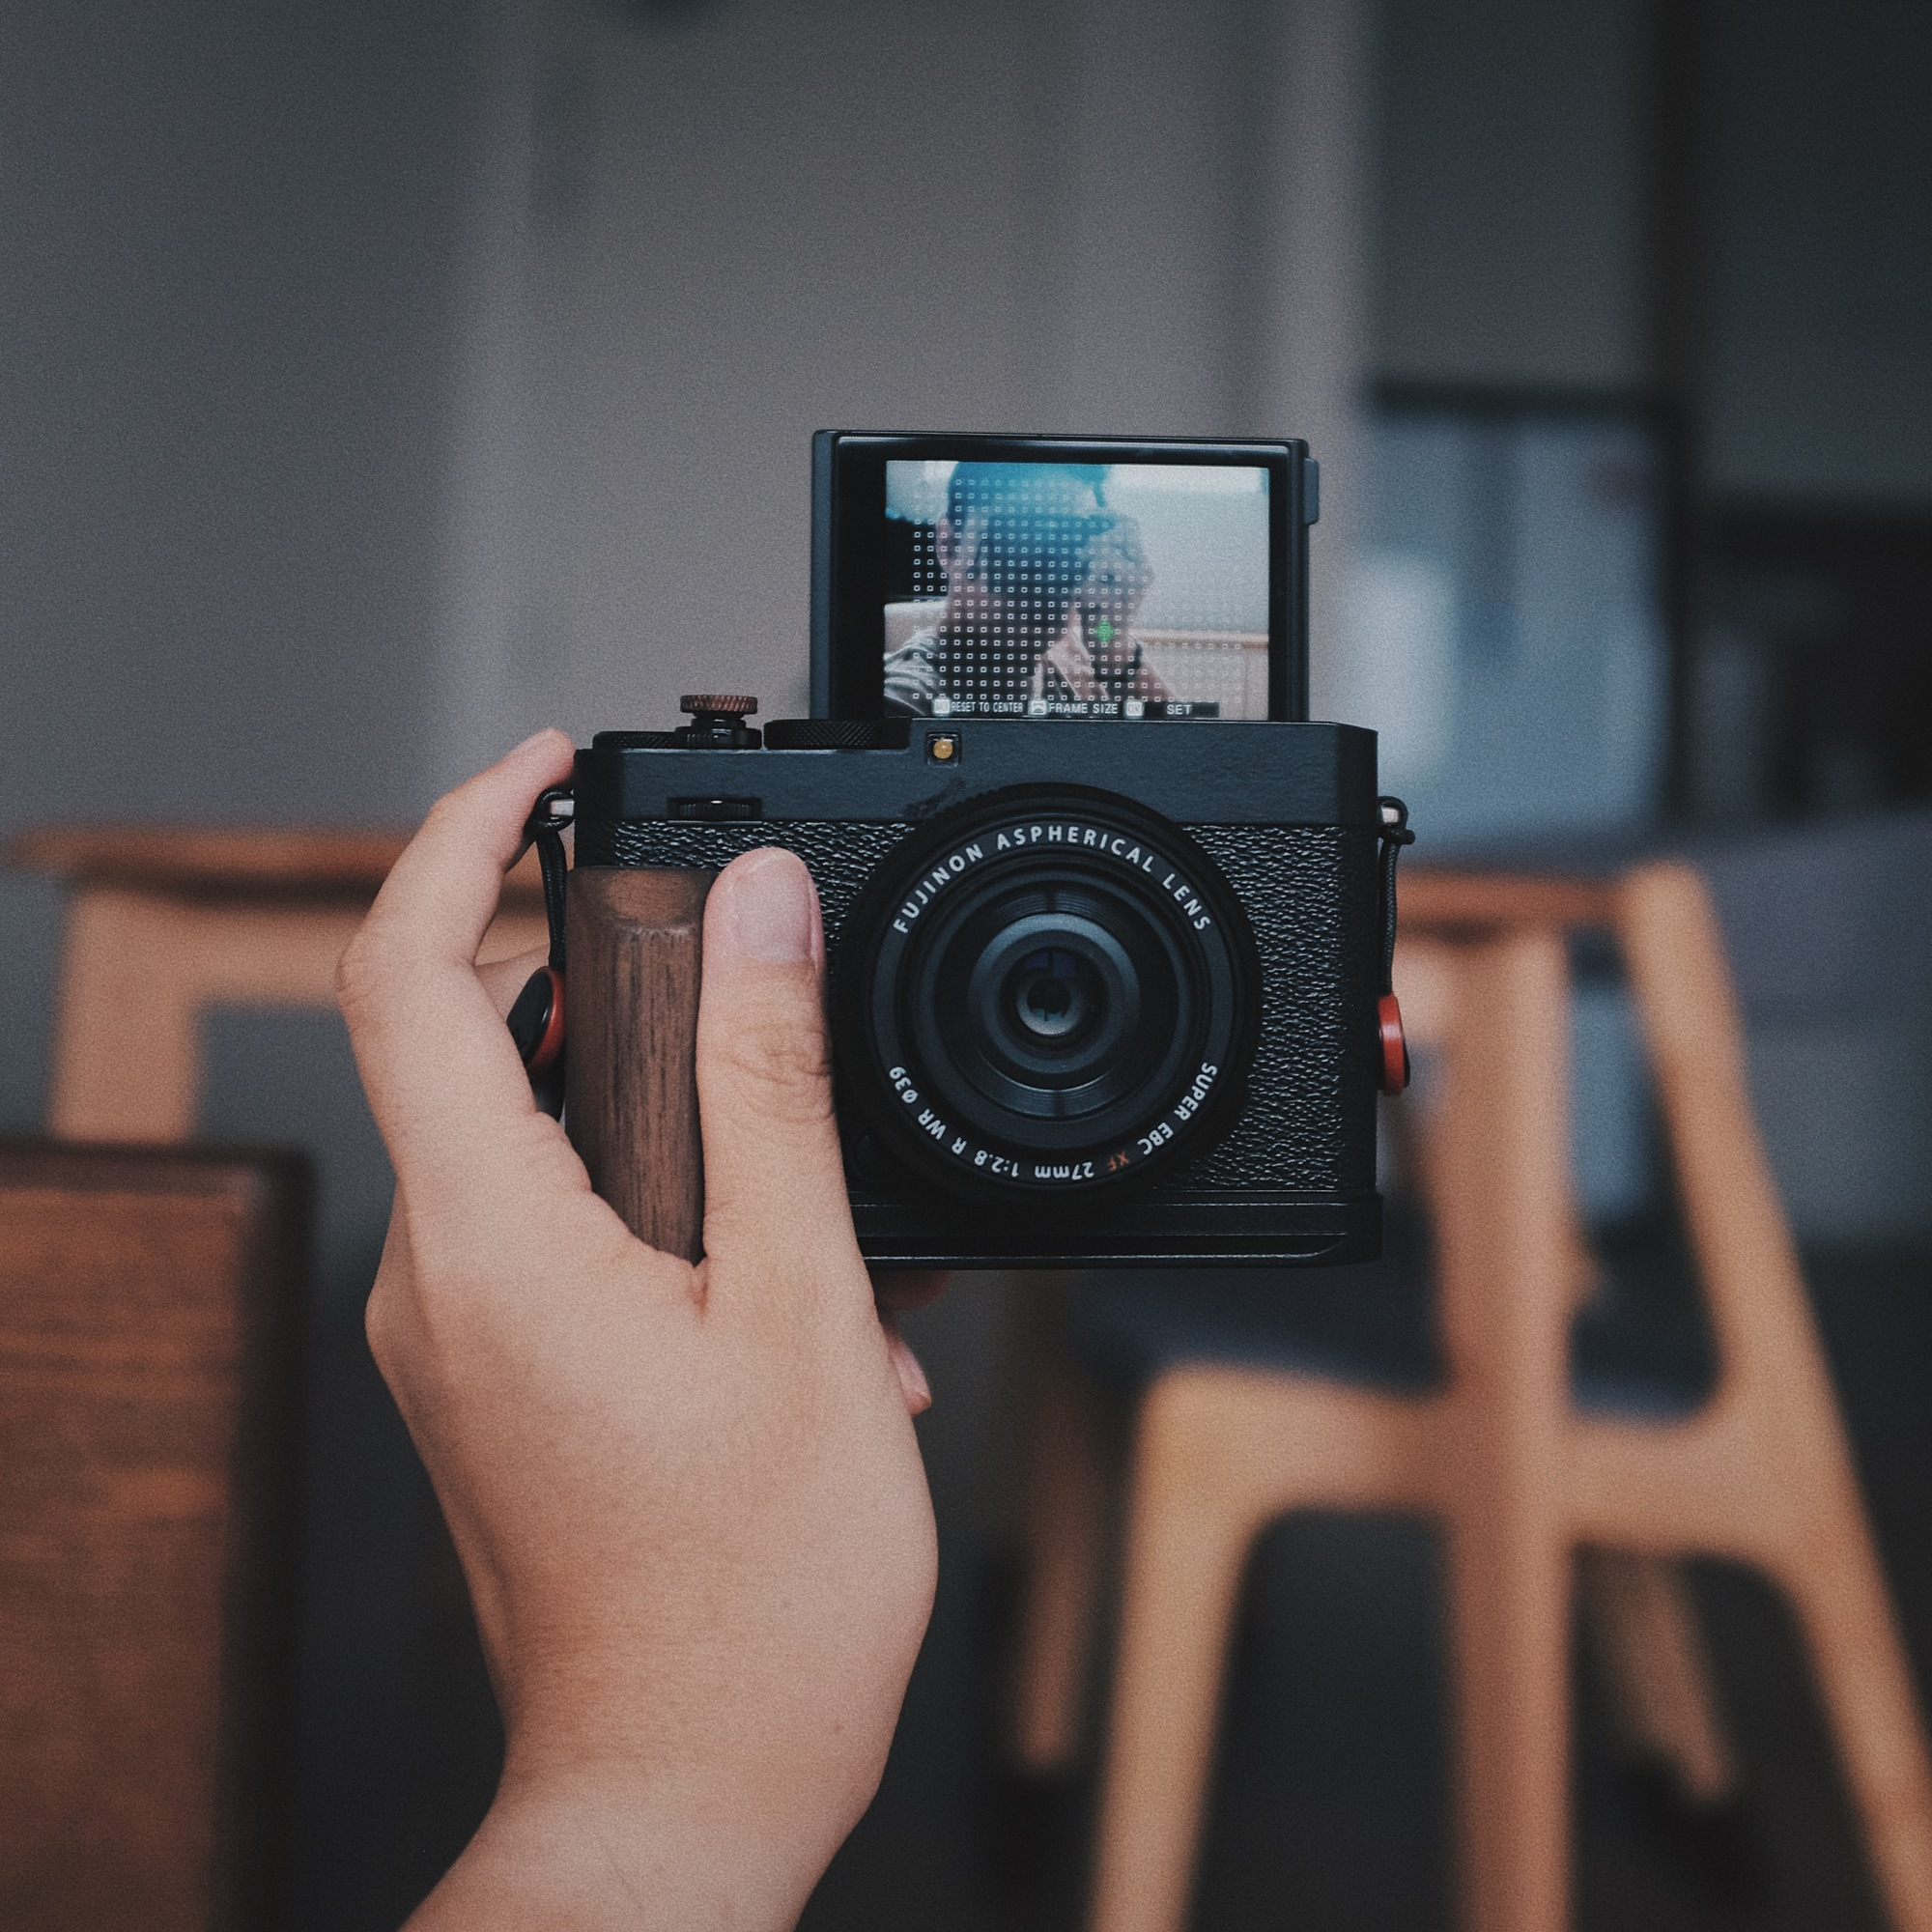
\includegraphics[width=\linewidth]{\envfinaldir/coverpic-prod.jpg}\par
            % \vskip 30pt
            \vfill

            \normalsize\rmfamily\scshape
            \copyright{} The Web Digest Project \hfill\large \envdatestr
        \end{center}
    \end{titlepage}
    % \restoregeometry
}
\newcommand{\simplehref}[1]{%
    \textcolor{blue!80!green}{\href{#1}{#1}}%
}
\renewcommand{\contentsname}{\center\Huge\sffamily\bfseries Contents\par\vskip 20pt}
\newcounter{ipartcounter}
\setcounter{ipartcounter}{0}
\newcommand{\ipart}[1]{
    % \vskip 20pt
    \clearpage
    \stepcounter{ipartcounter}
    \phantomsection
    \addcontentsline{toc}{chapter}{#1}
    % \begin{center}
    %     \Huge
    %     \sffamily\bfseries
    %     #1
    % \end{center}
    % \vskip 20pt plus 7pt
}
\newcounter{ichaptercounter}
\setcounter{ichaptercounter}{0}
\newcommand{\ichapter}[1]{
    % \vskip 20pt
    \clearpage
    \stepcounter{ichaptercounter}
    \phantomsection
    \addcontentsline{toc}{section}{\numberline{\arabic{ichaptercounter}}#1}
    \begin{center}
        \Huge
        \sffamily\bfseries
        #1
    \end{center}
    \vskip 20pt plus 7pt
}
\newcommand{\entrytitlefont}[1]{\subsection*{\raggedright\Large\sffamily\bfseries#1}}
\newcommand{\entryitemGeneric}[2]{
    % argv: title, url
    \parbox{\linewidth}{
        \entrytitlefont{#1}\par\vskip 5pt
        \footnotesize\ttfamily\mdseries
        \simplehref{#2}
    }\vskip 11pt plus 11pt minus 1pt
}
\newcommand{\entryitemGithub}[3]{
    % argv: title, url, desc
    \parbox{\linewidth}{
        \entrytitlefont{#1}\par\vskip 5pt
        \footnotesize\ttfamily\mdseries
        \simplehref{#2}\par\vskip 5pt
        \small\rmfamily\mdseries#3
    }\vskip 11pt plus 11pt minus 1pt
}
\newcommand{\entryitemAp}[3]{
    % argv: title, url, desc
    \parbox{\linewidth}{
        \entrytitlefont{#1}\par\vskip 5pt
        \footnotesize\ttfamily\mdseries
        \simplehref{#2}\par\vskip 5pt
        \small\rmfamily\mdseries#3
    }\vskip 11pt plus 11pt minus 1pt
}
\newcommand{\entryitemHackernews}[3]{
    % argv: title, hnurl, rawurl
    % \parbox{\linewidth}{
    %     \entrytitlefont{#1}\par\vskip 5pt
    %     \footnotesize\ttfamily\mdseries
    %     \simplehref{#3}\par
    %     \textcolor{black!50}{\href{#2}{#2}}
    % }\vskip 11pt plus 11pt minus 1pt
    \begin{minipage}{\linewidth}
            \entrytitlefont{#1}\par\vskip 5pt
            \footnotesize\ttfamily\mdseries
            \simplehref{#3}\par
            \textcolor{black!50}{\href{#2}{#2}}
    \end{minipage}\par\vskip 11pt plus 11pt minus 1pt
}







\begin{document}

\makeheader

\tableofcontents\clearpage




\ipart{Developers}
\ichapter{Hacker News}
\entryitemTwoLinks{Do not download the app, use the website}{https://news.ycombinator.com/item?id=44689059}{https://idiallo.com/blog/dont-download-apps}

\entryitemTwoLinks{It's time for modern CSS to kill the SPA}{https://news.ycombinator.com/item?id=44688489}{https://www.jonoalderson.com/conjecture/its-time-for-modern-css-to-kill-the-spa/}

\entryitemTwoLinks{Vanilla JavaScript support for Tailwind Plus}{https://news.ycombinator.com/item?id=44686317}{https://tailwindcss.com/blog/vanilla-js-support-for-tailwind-plus}

\entryitemTwoLinks{Animated Cursors}{https://news.ycombinator.com/item?id=44686164}{https://tattoy.sh/news/animated-cursors/}

\entryitemTwoLinks{Never write your own date parsing library}{https://news.ycombinator.com/item?id=44685875}{https://www.zachleat.com/web/adventures-in-date-parsing/}

\entryitemTwoLinks{Internet Archive is now a federal depository library}{https://news.ycombinator.com/item?id=44685342}{https://www.kqed.org/news/12049420/sf-based-internet-archive-is-now-a-federal-depository-library-what-does-that-mean}

\entryitemTwoLinks{Why MIT switched from Scheme to Python (2009)}{https://news.ycombinator.com/item?id=44685119}{https://www.wisdomandwonder.com/link/2110/why-mit-switched-from-scheme-to-python}

\entryitemTwoLinks{Efficient Computer's Electron E1 CPU – 100x more efficient than Arm?}{https://news.ycombinator.com/item?id=44685050}{https://morethanmoore.substack.com/p/efficient-computers-electron-e1-cpu}

\entryitemTwoLinks{Steam, Itch.io are pulling `porn' games. Critics say it's a slippery slope}{https://news.ycombinator.com/item?id=44685011}{https://www.wired.com/story/steam-itchio-are-pulling-porn-games-censorship/}

\entryitemTwoLinks{Women dating safety app 'Tea' breached, users' IDs posted to 4chan}{https://news.ycombinator.com/item?id=44684373}{https://www.404media.co/women-dating-safety-app-tea-breached-users-ids-posted-to-4chan/}

\entryitemTwoLinks{Programming vehicles in games}{https://news.ycombinator.com/item?id=44683682}{https://wassimulator.com/blog/programming/programming\_vehicles\_in\_games.html}

\entryitemTwoLinks{Google's shortened goo.gl links will stop working next month}{https://news.ycombinator.com/item?id=44683481}{https://www.theverge.com/news/713125/google-url-shortener-links-shutdown-deadline}

\entryitemTwoLinks{It's a DE9, not a DB9 (but we know what you mean)}{https://news.ycombinator.com/item?id=44682964}{https://news.sparkfun.com/14298}

\entryitemTwoLinks{Who has the fastest F1 website (2021)}{https://news.ycombinator.com/item?id=44682932}{https://jakearchibald.com/2021/f1-perf-part-3/}

\entryitemTwoLinks{Show HN: Price Per Token – LLM API Pricing Data}{https://news.ycombinator.com/item?id=44682465}{https://pricepertoken.com/}

\entryitemTwoLinks{The future is not self-hosted}{https://news.ycombinator.com/item?id=44682175}{https://www.drewlyton.com/story/the-future-is-not-self-hosted/}

\entryitemTwoLinks{Qwen3-235B-A22B-Thinking-2507}{https://news.ycombinator.com/item?id=44681565}{https://huggingface.co/Qwen/Qwen3-235B-A22B-Thinking-2507}

\entryitemTwoLinks{Games Look Bad: HDR and Tone Mapping (2017)}{https://news.ycombinator.com/item?id=44680547}{https://ventspace.wordpress.com/2017/10/20/games-look-bad-part-1-hdr-and-tone-mapping/}

\entryitemTwoLinks{Quantitative AI progress needs accurate and transparent evaluation}{https://news.ycombinator.com/item?id=44680308}{https://mathstodon.xyz/@tao/114910028356641733}

\entryitemTwoLinks{Google spoofed via DKIM replay attack: A technical breakdown}{https://news.ycombinator.com/item?id=44679854}{https://easydmarc.com/blog/google-spoofed-via-dkim-replay-attack-a-technical-breakdown/}


\ipart{Developers~~~~(zh-Hans)}
\ichapter{Solidot}
\entryitemGeneric{\hskip 0pt{}微软 CEO 轻淡的回应公司裁员之谜}{https://www.solidot.org/story?sid=81892}

\entryitemGeneric{\hskip 0pt{}Mistral AI 环境报告证实 AI 是一个饥渴的怪物}{https://www.solidot.org/story?sid=81891}

\entryitemGeneric{\hskip 0pt{}特朗普威胁关闭 TikTok }{https://www.solidot.org/story?sid=81890}

\entryitemGeneric{\hskip 0pt{}Debian 13.0 Trixie 的新变化}{https://www.solidot.org/story?sid=81889}

\entryitemGeneric{\hskip 0pt{}GPD 推出配备 Ryzen AI Max+ 395 的掌机}{https://www.solidot.org/story?sid=81888}

\entryitemGeneric{\hskip 0pt{}日本将允许用 iPS 细胞制造人类受精卵}{https://www.solidot.org/story?sid=81887}

\entryitemGeneric{\hskip 0pt{}英特尔今年将裁员 2.4 万人}{https://www.solidot.org/story?sid=81886}

\entryitemGeneric{\hskip 0pt{}2023 年的海洋热浪史无前例}{https://www.solidot.org/story?sid=81885}

\entryitemGeneric{\hskip 0pt{}CERN 演示反物质量子比特}{https://www.solidot.org/story?sid=81884}

\entryitemGeneric{\hskip 0pt{}国际法院认为健康环境是人权}{https://www.solidot.org/story?sid=81883}

\entryitemGeneric{\hskip 0pt{}Telegram 上的偷拍群组}{https://www.solidot.org/story?sid=81882}

\entryitemGeneric{\hskip 0pt{}FDA 的 AI 工具被发现捏造研究}{https://www.solidot.org/story?sid=81881}

\entryitemGeneric{\hskip 0pt{}硅谷 AI 创业公司拥抱中国的 996 工作制}{https://www.solidot.org/story?sid=81880}

\entryitemGeneric{\hskip 0pt{}图瓦卢逾八成国民寻求澳大利亚的气候移民签证}{https://www.solidot.org/story?sid=81879}

\entryitemGeneric{\hskip 0pt{}索尼通过降低 PS5 性能应对全球气候变化}{https://www.solidot.org/story?sid=81877}

\entryitemGeneric{\hskip 0pt{}AWS 关闭上海 AI 研究中心}{https://www.solidot.org/story?sid=81876}

\entryitemGeneric{\hskip 0pt{}英国将禁止公共部门向勒索软件组织支付赎金}{https://www.solidot.org/story?sid=81875}

\entryitemGeneric{\hskip 0pt{}Steam 之后 Itch.io 限制成人游戏}{https://www.solidot.org/story?sid=81874}

\entryitemGeneric{\hskip 0pt{}热浪下欧洲软化对空调的抵制}{https://www.solidot.org/story?sid=81873}

\entryitemGeneric{\hskip 0pt{}气候变化导致森林火灾日益常见}{https://www.solidot.org/story?sid=81872}\ichapter{V2EX}
\entryitemGeneric{\hskip 0pt{}[问与答] 如何将同事请吃饭的钱给她}{https://www.v2ex.com/t/1147799}

\entryitemGeneric{\hskip 0pt{}[搜索引擎优化] 我自己做了个网站,但是搜关键词,找不到我网站,应该怎么样把排名搞上去呢?}{https://www.v2ex.com/t/1147798}

\entryitemGeneric{\hskip 0pt{}[宽带症候群] 自带 DCO 模块的内核马上就要发布了,有在用这个模块的朋友吗?}{https://www.v2ex.com/t/1147797}

\entryitemGeneric{\hskip 0pt{}[分享创造] Raphael AI - AI Photo Editor,全球首款免费、免登录的图片编辑器, 只靠文字输入编辑图片}{https://www.v2ex.com/t/1147796}

\entryitemGeneric{\hskip 0pt{}[分享创造] [MD TO PNG] MarkoSnap - 让文字,被看见}{https://www.v2ex.com/t/1147795}

\entryitemGeneric{\hskip 0pt{}[分享发现] 网页浏览器安装了屏蔽拦截广告等插件有可能会导致浏览 B 站时获得如同 3g 时代一般的体验,,,这里说下我的很简单的变相解决方法}{https://www.v2ex.com/t/1147794}

\entryitemGeneric{\hskip 0pt{}[分享创造] 做了一个 markdown 转卡片的网站,希望大家给些建议}{https://www.v2ex.com/t/1147793}

\entryitemGeneric{\hskip 0pt{}[Docker] 在容器里运行 VPN,如何接管其他容器的流量作为默认出口?}{https://www.v2ex.com/t/1147792}

\entryitemGeneric{\hskip 0pt{}[酷工作] [深圳] Agent 前端开发工程师(1-3 年)}{https://www.v2ex.com/t/1147791}

\entryitemGeneric{\hskip 0pt{}[宽带症候群] 拉了电信,还有公网 IP,网游反而更卡顿了,会不会是物理线路的问题呢}{https://www.v2ex.com/t/1147790}

\entryitemGeneric{\hskip 0pt{}[macOS] 🐧又作妖,右键居然多了一个``用 QQ 闪传发文件''的菜单}{https://www.v2ex.com/t/1147789}

\entryitemGeneric{\hskip 0pt{}[Solana] [体验] 没玩过加密货币 想试一下被打赏。 买比特币也是用 phantom 钱包吗}{https://www.v2ex.com/t/1147787}

\entryitemGeneric{\hskip 0pt{}[Kubernetes] 有没有 k8s + ingress +frp 这种方案}{https://www.v2ex.com/t/1147786}

\entryitemGeneric{\hskip 0pt{}[分享发现] 论文写作辅助必备! 9 个超实用 AI 工具大揭秘~}{https://www.v2ex.com/t/1147785}

\entryitemGeneric{\hskip 0pt{}[Cursor] Cursor 不能用了啊,如何破啊,老铁们}{https://www.v2ex.com/t/1147784}

\entryitemGeneric{\hskip 0pt{}[macOS] Mac 版 Apple Music,按空格键会对加入资料库或播放列表的歌曲进行 收藏/取消收藏}{https://www.v2ex.com/t/1147783}

\entryitemGeneric{\hskip 0pt{}[推广] 大喵推出计算专业大学预科班,学费 2k 一百节课,好评如潮,错过等一年}{https://www.v2ex.com/t/1147782}

\entryitemGeneric{\hskip 0pt{}[分享创造] 「iMockup」- 给独立开发者和设计师用的 APP 样机模型动画工具}{https://www.v2ex.com/t/1147780}

\entryitemGeneric{\hskip 0pt{}[程序员] 微软也学坏了,拿着 edge 搞劫持这一套}{https://www.v2ex.com/t/1147776}

\entryitemGeneric{\hskip 0pt{}[宽带症候群] 火狐隐身模式老是异常流量}{https://www.v2ex.com/t/1147775}

\entryitemGeneric{\hskip 0pt{}[Solana] [体验]想收 0.01sol,拿来当 gas}{https://www.v2ex.com/t/1147773}

\entryitemGeneric{\hskip 0pt{}[问与答] 大家腾讯视频目前有内存泄露的情况吗}{https://www.v2ex.com/t/1147772}

\entryitemGeneric{\hskip 0pt{}[VXNA] 申请收录个人博客: zeratulqiu.me}{https://www.v2ex.com/t/1147771}

\entryitemGeneric{\hskip 0pt{}[摄影] 你见过会发光的沙丘嘛?}{https://www.v2ex.com/t/1147768}

\entryitemGeneric{\hskip 0pt{}[分享创造] How AI Influencers Are Making Money Using AI-Generated Models with ModelMaker.app}{https://www.v2ex.com/t/1147767}

\entryitemGeneric{\hskip 0pt{}[宽带症候群] 家里有两个小米摄像头云存储被联通限速了,说摄像头就是 PCDN}{https://www.v2ex.com/t/1147764}

\entryitemGeneric{\hskip 0pt{}[酷工作] [合作机会招募] 更易上手的 Claude Code 平替方案,助你降本增效!}{https://www.v2ex.com/t/1147763}

\entryitemGeneric{\hskip 0pt{}[酷工作] Web3 Dex 团队招聘资深前端开发工程师}{https://www.v2ex.com/t/1147762}

\entryitemGeneric{\hskip 0pt{}[分享发现] [开源分享] 鸿蒙沙箱浏览器 - SandboxFinder}{https://www.v2ex.com/t/1147761}

\entryitemGeneric{\hskip 0pt{}[CDN] CoverIP CDN 不成熟测评}{https://www.v2ex.com/t/1147760}

\entryitemGeneric{\hskip 0pt{}[Kubernetes] 各位公司生产环境操作系统容器镜像选型是什么?}{https://www.v2ex.com/t/1147759}

\entryitemGeneric{\hskip 0pt{}[问与答] 触控便携屏代替平板是否可行}{https://www.v2ex.com/t/1147758}

\entryitemGeneric{\hskip 0pt{}[以太坊] 复刻一个 etherscan.io 这样的网站需要多少钱?}{https://www.v2ex.com/t/1147757}

\entryitemGeneric{\hskip 0pt{}[游戏] 有没有什么好玩的冒险岛私服}{https://www.v2ex.com/t/1147756}

\entryitemGeneric{\hskip 0pt{}[Apple] macos 26 beta 4 怎么找回 spotlight 启动台图标?}{https://www.v2ex.com/t/1147755}

\entryitemGeneric{\hskip 0pt{}[加密货币] 不懂就问如何学习 web3 开发}{https://www.v2ex.com/t/1147754}

\entryitemGeneric{\hskip 0pt{}[Node.js] 比 prisma studio 更好性能的类 studio 数据管理}{https://www.v2ex.com/t/1147752}

\entryitemGeneric{\hskip 0pt{}[程序员] MoonBit 又开始搞全球编程挑战赛了,这次双赛道 + 高额奖励}{https://www.v2ex.com/t/1147751}

\entryitemGeneric{\hskip 0pt{}[Docker] docker 重磅安全漏洞}{https://www.v2ex.com/t/1147750}

\entryitemGeneric{\hskip 0pt{}[生活] 屋漏偏逢连夜雨,女友跑了,十字韧带又断了}{https://www.v2ex.com/t/1147748}

\entryitemGeneric{\hskip 0pt{}[iDev] 多个开发者账号,会被关联吗}{https://www.v2ex.com/t/1147747}

\entryitemGeneric{\hskip 0pt{}[宽带症候群] 求助:2.5G 网卡宽带只能跑到 300M 可能是什么原因?}{https://www.v2ex.com/t/1147746}

\entryitemGeneric{\hskip 0pt{}[Apple] 16PM 与折叠屏选择}{https://www.v2ex.com/t/1147745}

\entryitemGeneric{\hskip 0pt{}[酷工作] [广州-三七互娱-社招内推]前端开发工程师}{https://www.v2ex.com/t/1147743}

\entryitemGeneric{\hskip 0pt{}[Solana] 都在空投 sol,那我跟风空投点\$V2EX 试试水吧}{https://www.v2ex.com/t/1147742}

\entryitemGeneric{\hskip 0pt{}[酷工作] base 深圳南山内推中高级安卓研发岗,流程快,不卡行业经验}{https://www.v2ex.com/t/1147741}

\entryitemGeneric{\hskip 0pt{}[程序员] Claude Code Sub-Agents:从手工作坊到自动化工厂}{https://www.v2ex.com/t/1147740}

\entryitemGeneric{\hskip 0pt{}[Solana] pump 中的 DB, DS dev bought/sold 是什么意思 指的是谁呢}{https://www.v2ex.com/t/1147739}

\entryitemGeneric{\hskip 0pt{}[问与答] B zhan 大会员收购一枚}{https://www.v2ex.com/t/1147738}

\entryitemGeneric{\hskip 0pt{}[Cursor] Cursor 额度用完了,这个月的后续工作怎么办}{https://www.v2ex.com/t/1147737}


\ipart{Generic News}







\clearpage
\leavevmode\vfill
\footnotesize

Copyright \copyright{} 2023-2025 Neruthes and other contributors.

This document is published with CC BY-NC-ND 4.0 license.

The entries listed in this newsletter may be copyrighted by their respective creators.

This newsletter is generated by the Web Digest project.

The newsletters are also delivered via Telegram channel \CJKunderline{\href{https://t.me/webdigestchannel}{https://t.me/webdigestchannel}}.\\
RSS feed is available at \CJKunderline{\href{https://webdigest.pages.dev/rss.xml}{https://webdigest.pages.dev/rss.xml}}.

This newsletter is available in PDF at
\CJKunderline{\href{https://webdigest.pages.dev/}{https://webdigest.pages.dev/}}.

The source code being used to generate this newsletter is available at\\
\CJKunderline{\href{https://github.com/neruthes/webdigest}{https://github.com/neruthes/webdigest}}.

This newsletter is also available in
\CJKunderline{\href{http://webdigest.pages.dev/readhtml/\envyear/WebDigest-20250726.html}{HTML}} and
\CJKunderline{\href{https://github.com/neruthes/webdigest/blob/master/markdown/\envyear/WebDigest-20250726.md}{Markdown}}.


\coverpic{https://unsplash.com/photos/sandy-dunes-create-rippled-patterns-in-the-desert-16t-HIIrWDI}{Waldemar}


\end{document}
